\chapter{Annotation~Experiments}
\label{chap:annotation} 

In this chapter I attempt to evaluate the annotation method as a whole. By using the tool to evaluate real datasets (described in chapter-\ref{chap:datasets}). 


\section {Evaluation method}




User edits are logged, along with predictions provided by the model (the starting point for annotating each image), and the final set of annotations submitted by the user. The accuracy of detections are verified directly by the user, giving both continuous testing of the model predictions as well as providing useful feedback to the user of the system. The types of actions as well as the timing can provide useful clues as to the difficulty of the task, and the level of assistance provided.

Concurrently, training statistics are logged, and the validation set (by default one in five images submitted) provides feedback as to the overall accuracy of the model on the particular task.



\section{Case Study: Counting Adelie Penguins}

One potentially useful for verification based annotation is counting things, it provides some of the time savings of automatic inference but also the accuracy of human annotation because the machine predictions are verified, and can begin without possessing an existing dataset or recognition algorithm.


One of the sources of inspiration for this work in verification based annotation came from \cite{McNeill2011}, where a tool was created to semi-automatically count Adelie penguins from aerial photographs. The penguins are first automatically detected, then follows a verification process allowing a human annotator to mark false positives and false negatives.

The method for detecting penguins is to first detect penguin colonies which can be done many times by the unique colour of the penguin guano. Individual penguins were then identified by thresholding and local minima detection and culling of long thin objects. 

The images (two of which can be seen in figure \ref{fig:penguin_examples}), originate from aerial photographic surveys \cite{Lyver2014}, from high resolution photographs, taken from 2000-2500 feet. In the case of the two images from Cape Cotter and Hallet in figure \ref{fig:penguin_examples}, the images are cropped from images of size $ 6720\times4480 $. The Cape Royds images are spliced together from three images with various areas masked out, this was done by filling in the overlapping and irrelevant areas using a paint program.

The study which has been conducted from 1981 until present, prior to 2010 involved manually counting individual penguins using a pin to manually mark penguins and avoid duplication. 

\begin{figure*}[h!]
\centering
\begin{subfigure}[t]{1.0\linewidth}
  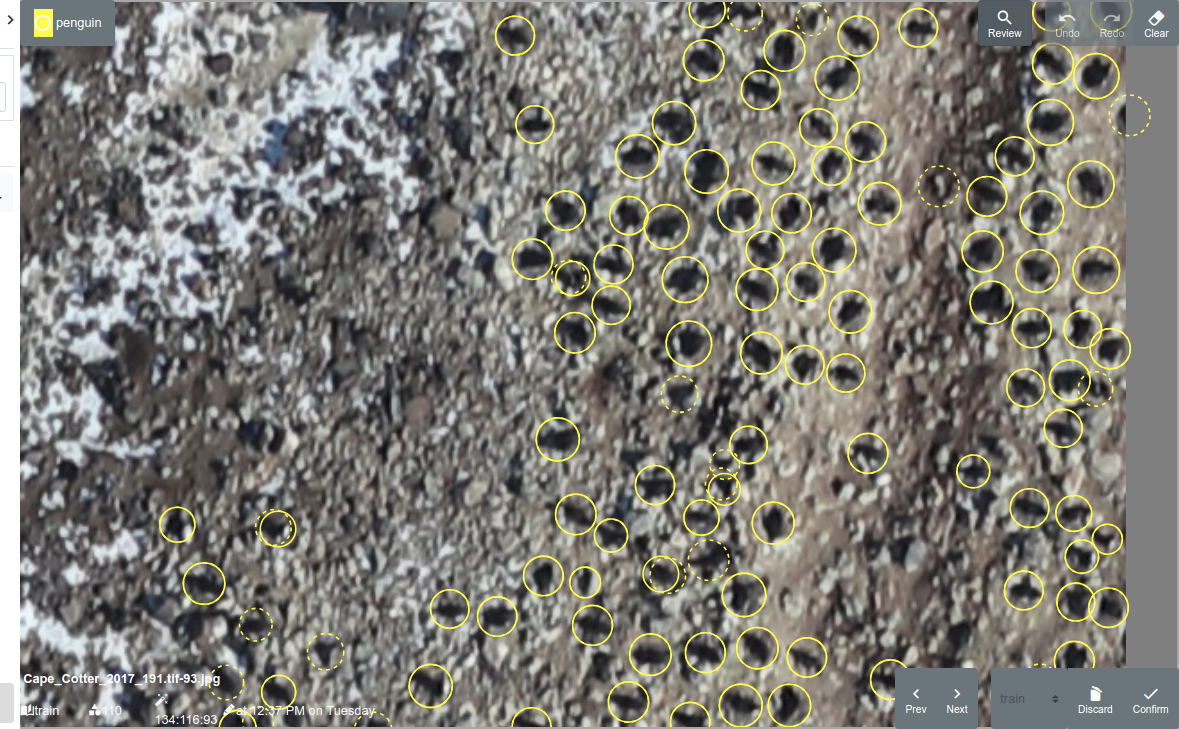
\includegraphics[width=0.475\linewidth]{figures/annotation/screenshots/penguins_aerial.png}
  \hfill
  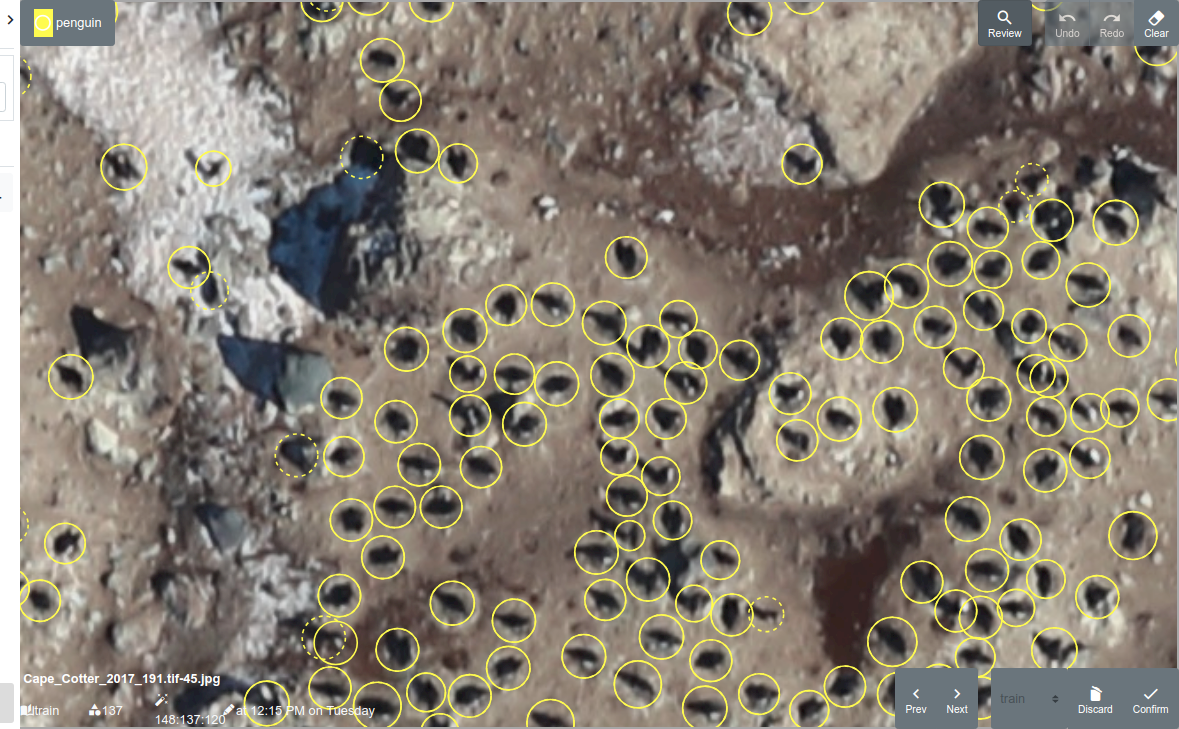
\includegraphics[width=0.475\linewidth]{figures/annotation/screenshots/penguins_aerial2.png}
  \caption{}
\end{subfigure}

\caption{ }
\label {fig:penguin_aerial_examples}
\end{figure*}



\begin{figure*}[h!]
\centering
\begin{subfigure}[t]{1.0\linewidth}
  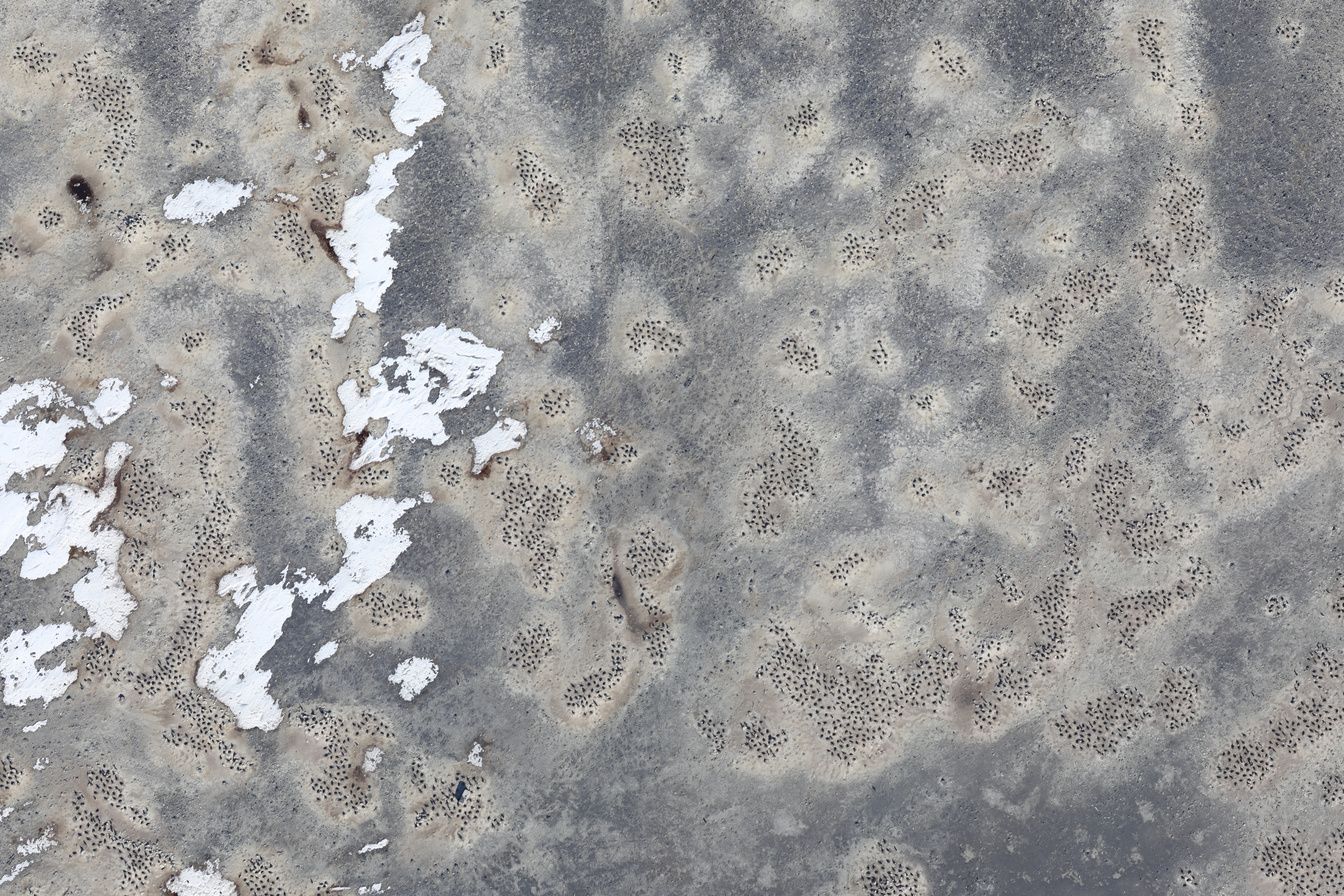
\includegraphics[width=0.475\linewidth]{figures/annotation/penguin/hallet_large.jpg}
  \hfill
  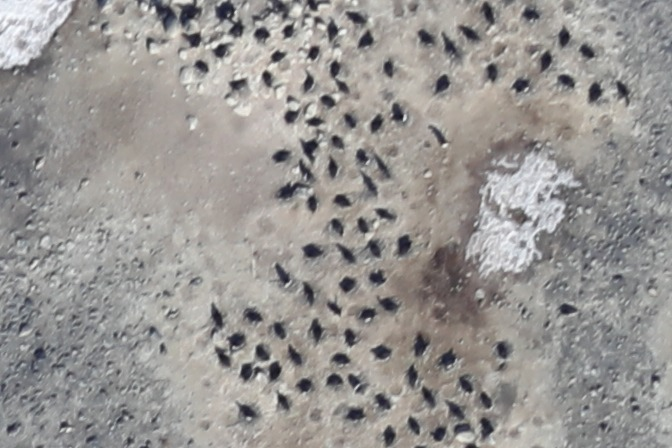
\includegraphics[width=0.475\linewidth]{figures/annotation/penguin/hallet.jpg}
  \caption{Cape Hallett 2017}
\end{subfigure}
\begin{subfigure}[t]{1.0\linewidth}
  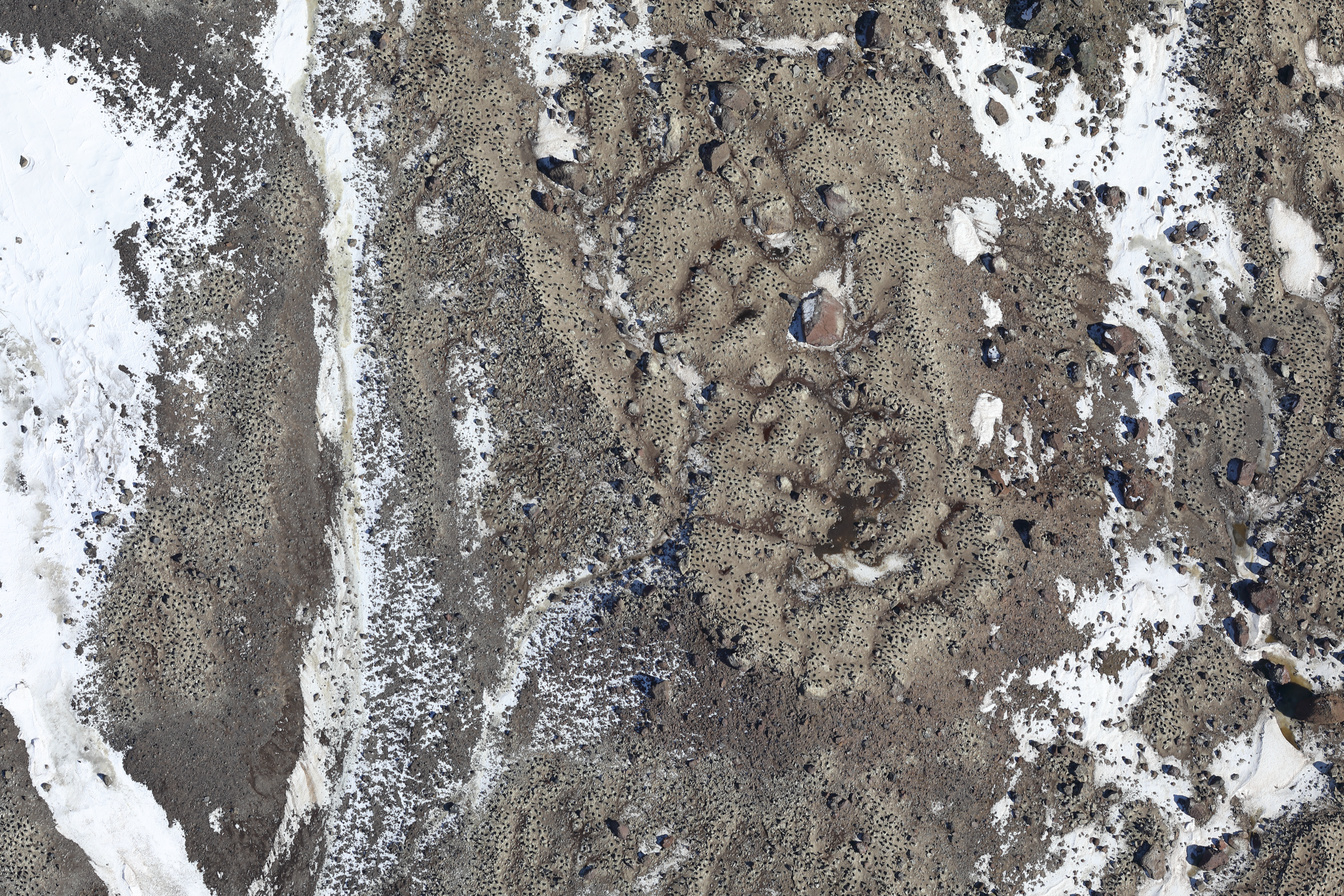
\includegraphics[width=0.475\linewidth]{figures/annotation/penguin/cotter_large.jpg}
  \hfill 
  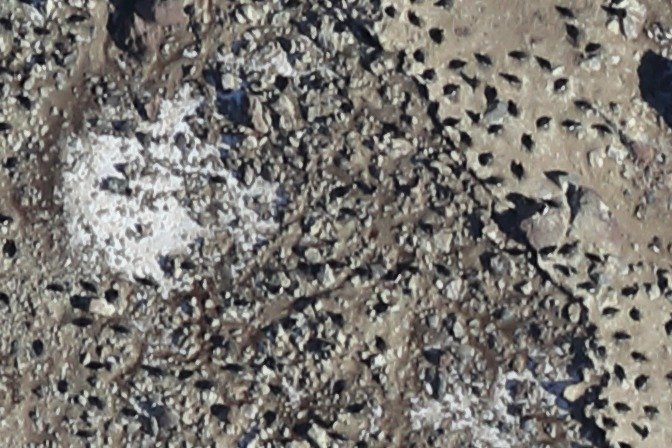
\includegraphics[width=0.475\linewidth]{figures/annotation/penguin/cotter.jpg}
  \caption{Cape Cotter 2017}
\end{subfigure}
\begin{subfigure}[t]{1.0\linewidth}
  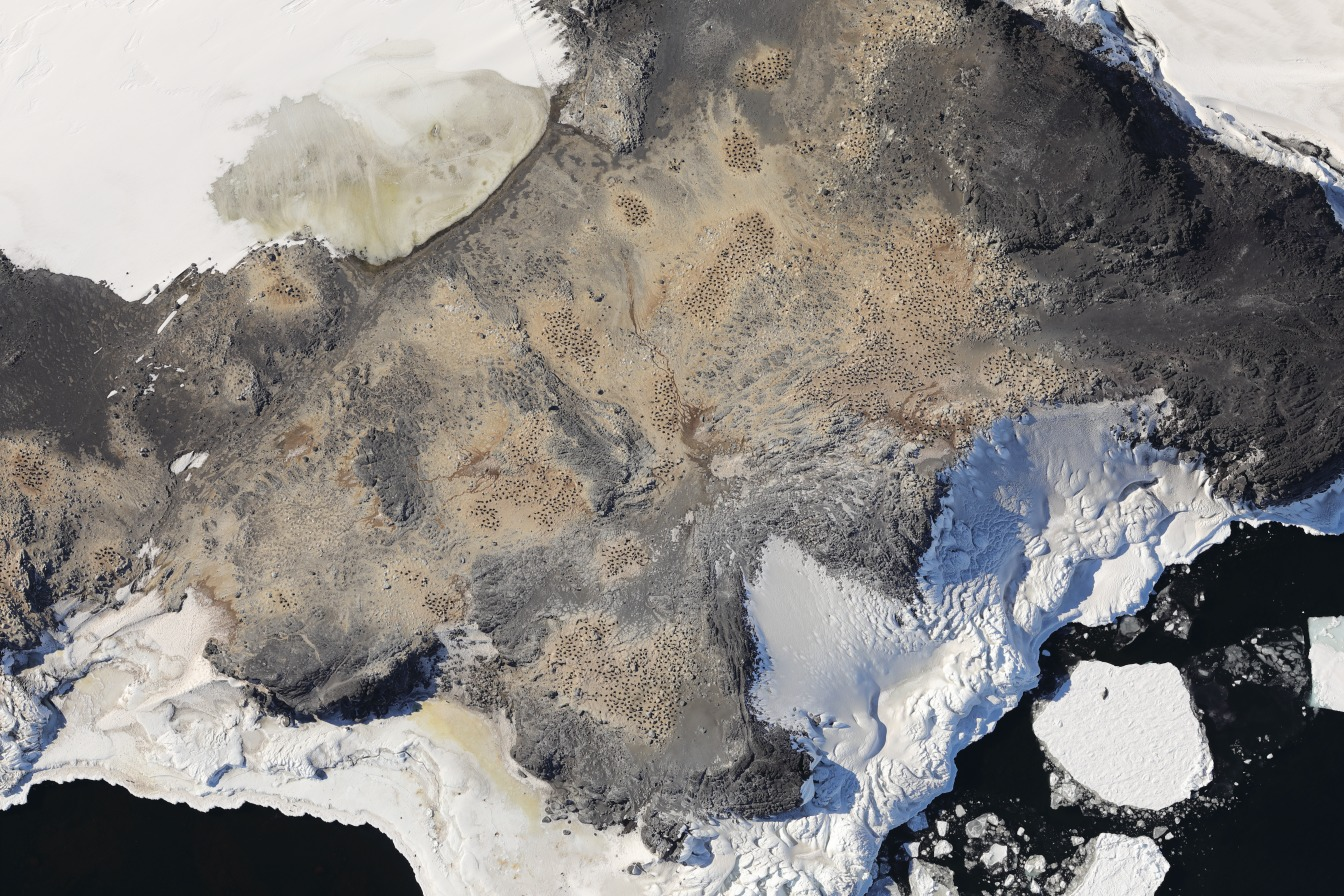
\includegraphics[width=0.475\linewidth]{figures/annotation/penguin/royds_large.jpg}
  \hfill
  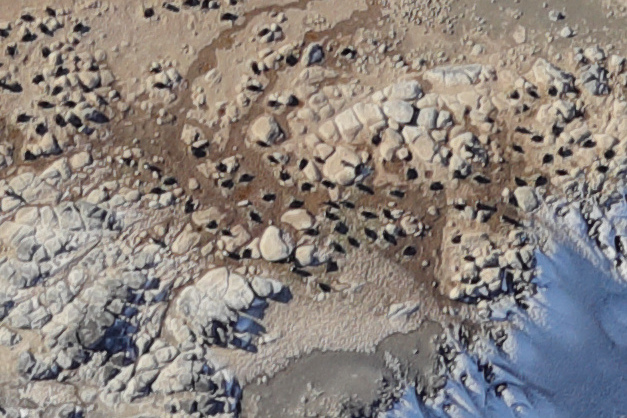
\includegraphics[width=0.475\linewidth]{figures/annotation/penguin/royds.jpg}
  \caption{Cape Royds 2017}
\end{subfigure}

\caption{Examples from the Adelie penguin census data taken in 2017. On the left hand column are images showing the zoomed out landscape, on the right are representative crops zoomed in.  In (a) an image from Cape Hallet image showing clearly visible, easy to identify penguins as dark patches. In (b) Cape Cotter showing many more difficult to identify penguins, often with a high degree of ambiguity not only for the machine learning algorithm but for a human annotator, in rocky areas especially shadows from rocks are very difficult to discern from penguins. In (c) Cape Royds, a smaller colony to the other two (and complete). In terms of ambiguity and uncertainty somewhere in-between. }
\label {fig:penguin_examples}
\end{figure*}


\subsection {Effect of uncertainty}

 The strength of the object detector has an effect on the usefulness of verification. If a detector is weak and the noise of many inaccurate detections overwhelms the number of any accurate detections, verification becomes less effective - and manual annotation becomes more efficient. When the source images are very uncertain this presents a challenge not only for the object detector which may be relatively weaker as a result, but for the human annotator. Many of the penguin instances to the untrained eye appear very similar to the shadow cast by rocks and difficult to discern. The nature of the imagery from the different sites shown in figure \ref{fig:penguin_examples} provide a test case to compare the effectiveness of verification with different levels of uncertainty in the source image. 

\subsection {Method}

Separately I annotated the three sets of penguins using the annotation tool. I used circular annotations as the precise location of the penguins is of no consequence for counting applications, and in general the penguins separate themselves with a wide berth (when viewed from above).  

The very large original images were split into images of size $ 672\times448 $ (Cape Royds images were of similar size, but not exactly the same because the source images were of different size, rather than one big image like the other two). Image crops of those image, sized $ 300\times300 $ were then used during training.

\begin{table}[ht]
  \centering
    \caption{Statistics from the thee penguin sources. }
  \begin{tabular}{ l  l  l  l  l }
    Image set & Total & Images & Validation & $AP_0.5$ \\
    \toprule
    Cape Hallett  & 4217 & 100 & 683 & 0.97 \\
    Cape Cotter   & 6180 & 100 & 973 & 0.72  \\
    Cape Royds    & 2754 & 61 & 477  & 0.88 \\
    \bottomrule
  \end{tabular}

\label{fig:penguin_statistics}
\end{table}





\subsection{Results and discussion}
 
The difference in difficulty can clearly be seen in the difference of mAP in figure \ref{fig:penguin_statistics}, where the Cape Hallet penguins were detected with almost perfect accuracy, whereas Cape Royds was more difficult and Cape Cotter considerably more difficult. 






\subsection{Counting accuracy}

The two images used in the previous section were sourced from larger colonies, here I annotate images from a small, but complete colony, where I can evaluate the accuracy of a fully automatic count as well as compare with the official count. The images above were at either extreme of difficulty, the images used in this section are somewhere in-between. 



\subsection{Case Study: Analysing Waddell Seal Counts}



\begin{figure*}[h!]
\centering
\begin{subfigure}[t]{1.0\linewidth}
  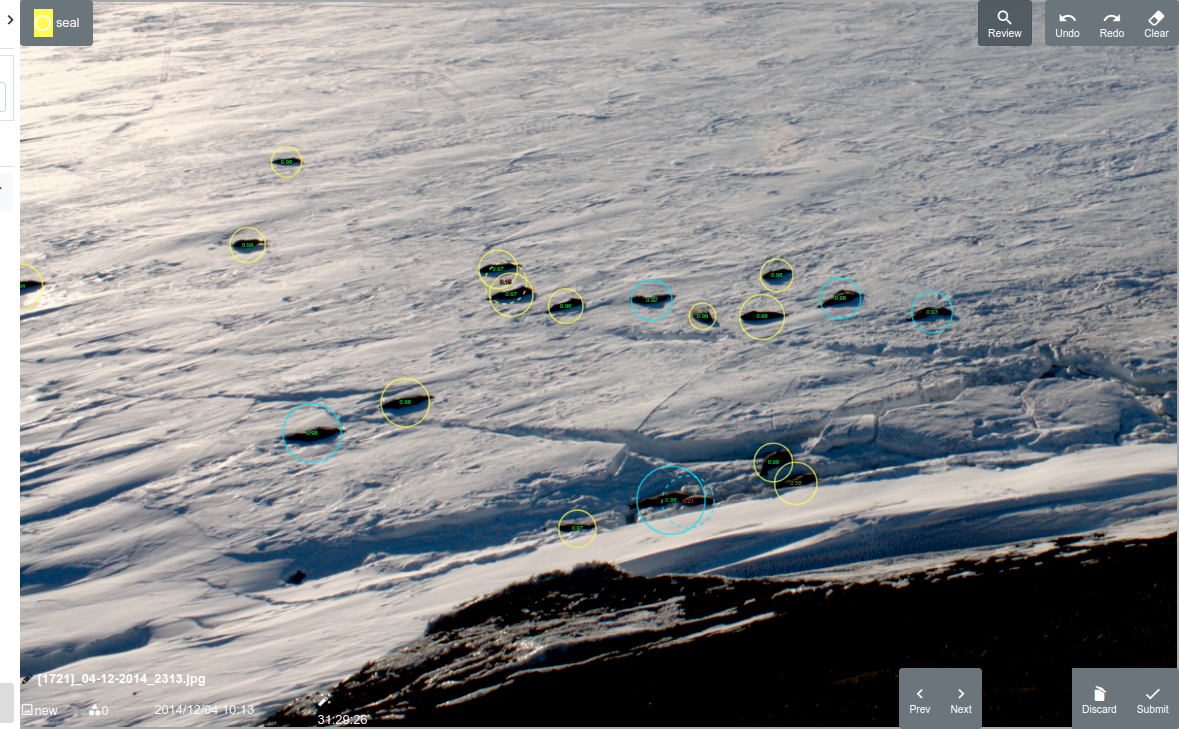
\includegraphics[width=0.475\linewidth]{figures/annotation/screenshots/seals_small2.png}
  \hfill
  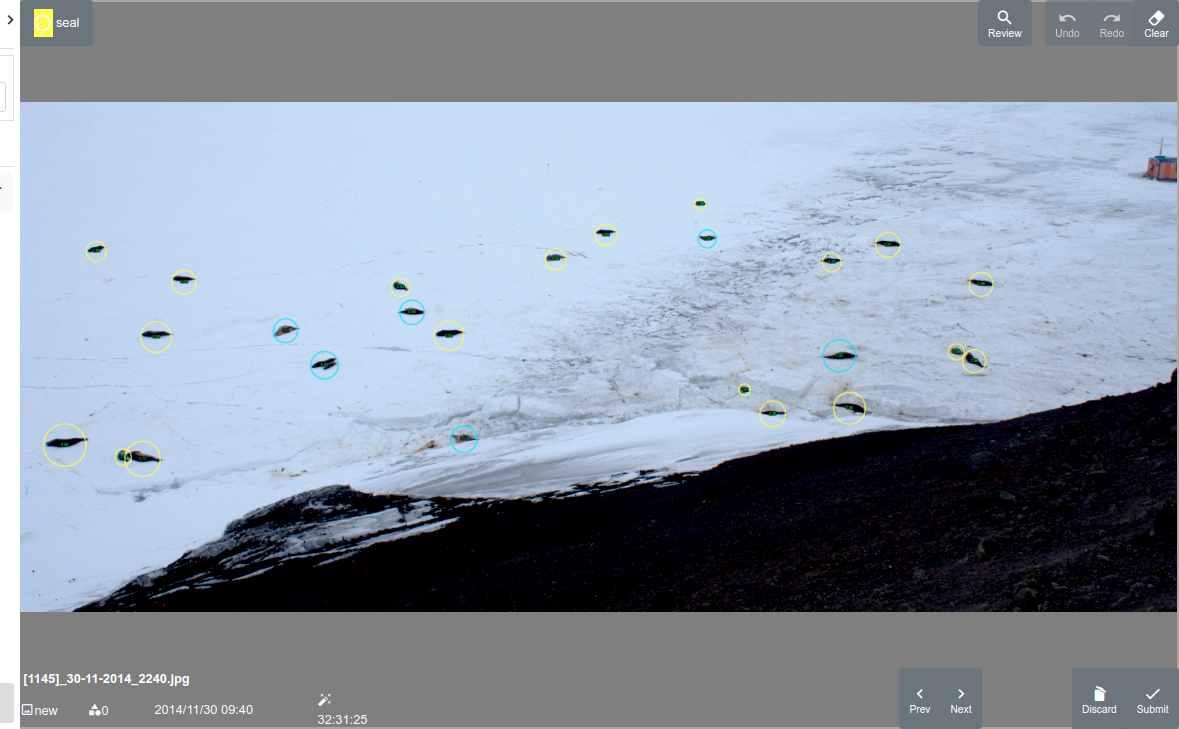
\includegraphics[width=0.475\linewidth]{figures/annotation/screenshots/seals_small.png}
  \caption{}
\end{subfigure}

\begin{subfigure}[t]{1.0\linewidth}
  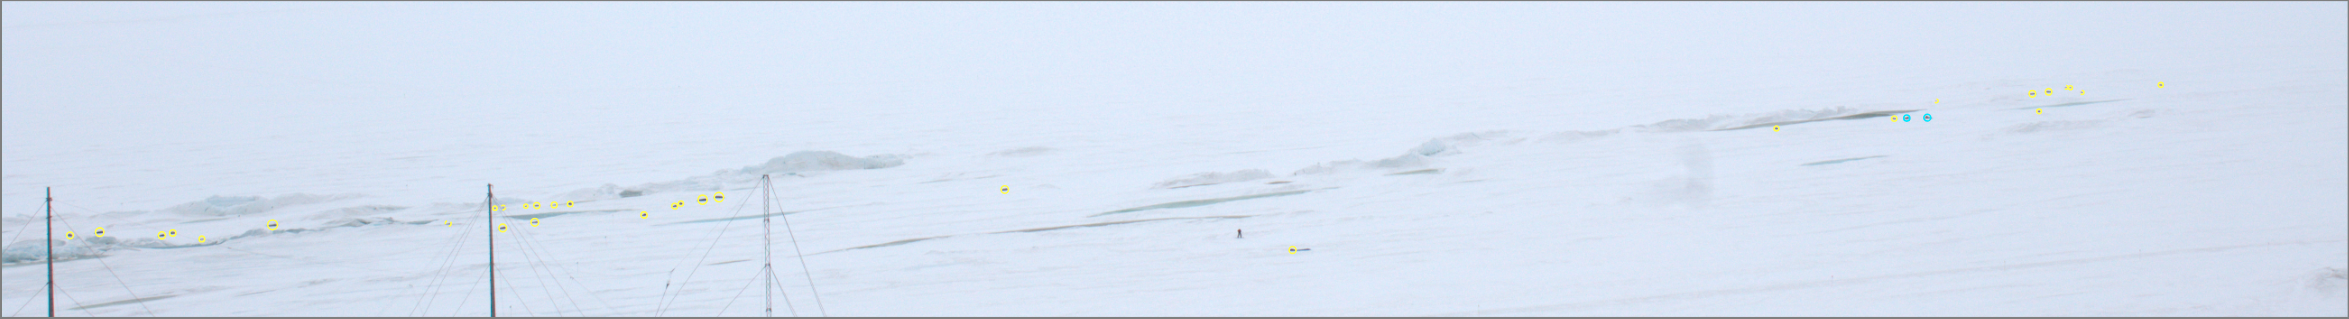
\includegraphics[width=1.0\linewidth]{figures/annotation/screenshots/cam_c.png}
\end{subfigure}

\begin{subfigure}[t]{1.0\linewidth}

  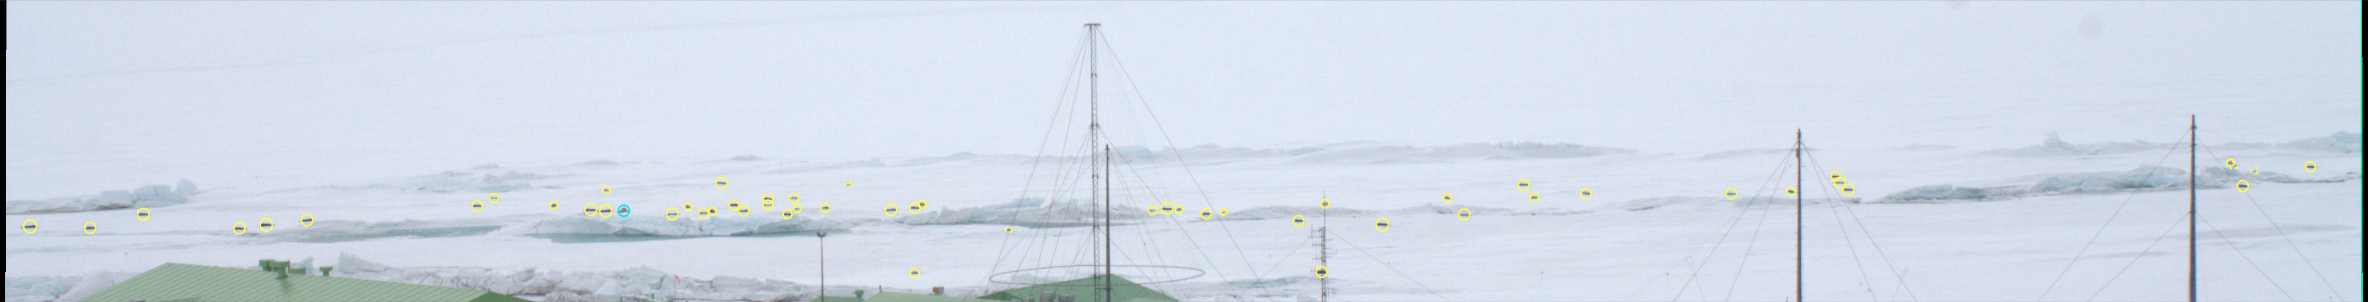
\includegraphics[width=1.0\linewidth]{figures/annotation/screenshots/cam_b.png}
  \caption{}
\end{subfigure}



\caption{ }
\label {fig:weddell_images}
\end{figure*}



